\documentclass[french]{article}
\usepackage[T1]{fontenc}
\usepackage{a4wide}
\usepackage{graphicx}
\usepackage{amssymb}
\usepackage{color}
\usepackage{babel}
\usepackage{hyperref}
\usepackage{amsmath}
\usepackage{cleveref}
\usepackage{comment}
\usepackage[utf8]{inputenc}
\usepackage{subcaption}

\providecommand{\tightlist}{%
  \setlength{\itemsep}{0pt}\setlength{\parskip}{0pt}}

\begin{document}

\begin{figure}[t]
\centering

\includegraphics[width=5cm]{rapport/inp_n7.png}
\end{figure}

\title{\vspace{4cm} \textbf{Projet Applications Web \\ Volundr}}
\author{Absobel\\ Pisenti Téo\\ Blot Olivier\\ Bru Louis\\ }
\date{\vspace{7cm} Département Sciences du Numérique - Deuxième année \\
2023-2024 }

\maketitle

\newpage

\section{Introduction}

    L'objectif de notre application $Volundr$ est de proposer une solution au problème de l'affectation de créneaux horaires à des élèves ou groupes d'élèves, par exemple lors d'examens oraux nécessitant un jury occupant une salle donnée pendant un certain nombre de créneaux horaires.


\section{Exemple de l'examen d'Applis Web}

    La problématique du passage à l'oral de cet examen est de faire passer des élèves de filières différentes (A,B,L,...) qui ont tous un emploi du temps différent.\\
    
    Dans un premier temps, le ou les professeurs jury rempliront leurs disponibilités à l'aide de la page présentée en \autoref{fig:modif_event}. En effet, il est possible pour un professeur de créer un événement (examen, présentation, suivi, ...) et d'y inviter des élèves et de préciser ses disponibilités en ajoutant des salles puis des créneaux. Pour ajouter un créneau, il faut rentrer le nombre de minutes souhaité pour la durée du créneau, cliquer sur "ajouter un créneau" pour enfin pouvoir sélectionner dans la colonne réprésentant la salle l'horaire de départ du créneau. Le professeur peut aussi renseigner une date de début et de fin pour les inscriptions des élèves. Un fois la durée des inscriptions expirée, le professeur peut cliquer sur "exécuter l'algorithme" pour lancer un algorithme d'affectation qui attribuera à chaque case un élève.\\
    
    Du côté des élèves, ils pourront (individuellement ou sous la forme d'un groupe) noter chaque créneau horaire mis à disposition par le professeur. Ici, comme nous pouvons le voir dans la \autoref{fig:choix_util}, le système de notation est composé de trois états : "oui", "peut-être" et "non". Pour noter une case, l'élève doit cliquer sur l'état voulu puis sur la case. Une fois que le professeur aura éxécuté l'algorithme d'affectation, les élèves auront accès au créneau qui leur a été attribué dans la liste de leurs événements.
    \\

\begin{comment}
    
\section{Schéma de données}

    \begin{figure}[h]
        \centering
        \includegraphics[width=12cm]{schema_donnees.png}
        \caption{Schéma de données}
        \label{fig:schema_donnees}
    \end{figure}

    \begin{enumerate}
        \item Case :\\
        Pour ce projet, nous avons décidé d'appeler $Case$ l'entity correspondant à un créneau horaire et la salle qui lui est associée. Une case est appartient à un seul événement, est accessible à plusieurs usagers qui peuvent chacun émettre un choix.
        
        \item Usager :\\
        Un usager représente tout type d'utilisateur. Il fait partie d'un établissement, et éventuellement d'un ou plusieurs groupes. Il lui est possible d'effectuer un choix sur une des cases auquelles il a accès.
        
        \item Choix :\\
         Un choix est matérialisé sous la forme d'une note, attribuée à une case par un usager.
         
        \item Salle :\\
         Une salle est représentée par un numéro ainsi qu'un nom de bâtiment, et appartient à un établissement. Une salle contient des cases qui ne sont pas forcément toutes réliées au même événement.
        \item Établissement :\\
        Un établissement est un regroupement de salles et d'usagers.
        
        \item Groupe :\\
        Un groupe contient un ou plusieurs usagers. Un groupe peut être invité à participer à plusieurs événements.
        
        \item Événement :\\
        Un événement représente une épreuve créée par un professeur par exemple. A la création d'un événement, des groupes sont invités à y participer, et des cases seront définies afin de permettre aux participants de formuler leurs choix.
        
    \end{enumerate}
\end{comment}

\section{Architecture du projet}

\subsection{Executer le projet}\label{executer-le-projet}

Le projet utilise maven pour télécharger automatiquement les dépendances
et générer le .war. On utilise wildfly (version communautaire et
maintenue de JBoss) comme serveur. Lancer \texttt{mvn\ build} pour
générer le .war Lancer \texttt{mvn\ wildfly:deploy} pour build et
déployer automatiquement dans wildfly

\subsection{Architecture du projet}\label{architecture-du-projet}

\subsubsection{Les packages Java du back-end sont dans ``src/main/java'' :}

\begin{itemize}
\tightlist
\item
  \textbf{package model :} Entities beans pour l'interaction avec la base de
  donnée
\item
  \textbf{package controller~:} L'interface entre le front et le back :

  \begin{itemize}
  \tightlist
  \item
    \textbf{Rest.java :} La définition de l'API REST utilisée par le front-end
    web au travers de la fonction ``fetch'' de JavaScript. Elle peut
    être testée avec curl avec les exemples suivants:
 \begin{verbatim}
# créer un utilisateur
curl -XPOST -H "Content-type: application/json" \
-d '{"mail": "teo@gmail.com", "prenom": "teo", "nom":"p" }' \
'http://localhost:8080/Volundr/rest/tutorial/addUser'
# récupérer la liste de tous les utilisateurs de la bdd
curl "http://localhost:8080/Volundr/rest/tutorial/getUsers"
\end{verbatim}
\item
    \textbf{Serv.java :} Une servlet utilisée par quelques rares pages web qui
    n'ont pas eu le temps d'être réécrites pour utiliser l'api REST
  \end{itemize}

\item
  \textbf{package dataTransfert :} Classes POJO qui servent à représenter les
  entities beans lors des communications entre le back et le front. Ce
  sont des copies des classes du modèle sans les attributs qu'on ne veut
  pas envoyer au client. Elles sont automatiquement sérialisées en JSON
  par l'API REST lors des réponses au client.

\end{itemize}

\subsubsection{Le code du front-end est dans src/main/webapp :}

Vous y trouverez du code jsp qui sert uniquement à générer du code HTML
car on utilise pas de framework de front-end comme React pour le faire. Par exemple: on l'utilise pour
inclure des fichiers html externes sans devoir copier coller le code
dans chaque fichier html.

Pour pouvoir être intéractives, les pages générées utilisent l'API REST
pour interragir avec le back-end grâce à la fonction ``fetch'' de
JavaScript.

Le dossier ``src/main/webapp/webscheduler'' contient un composant
permettant d'avoir une nouvelle balise html ``volundr-scheduler'' pour
gérer l'emploi du temps. Ce widget est écrit ``from scratch'' avec
uniquement du HTML,CSS,JS avec l'api ``webcomponent''.

\newpage

\section{Annexes}

    \begin{figure}[h]
        \centering
        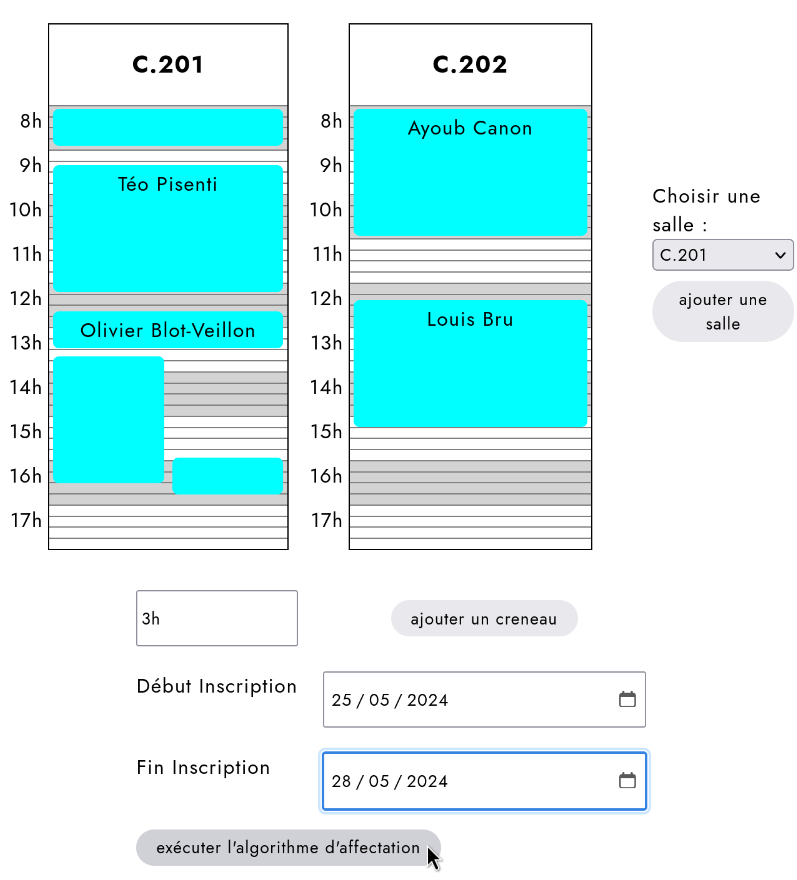
\includegraphics[width=8cm]{rapport/modif_event.png}
        \caption{Configuration d'un événement par un admin}
        \label{fig:modif_event}

        \centering
        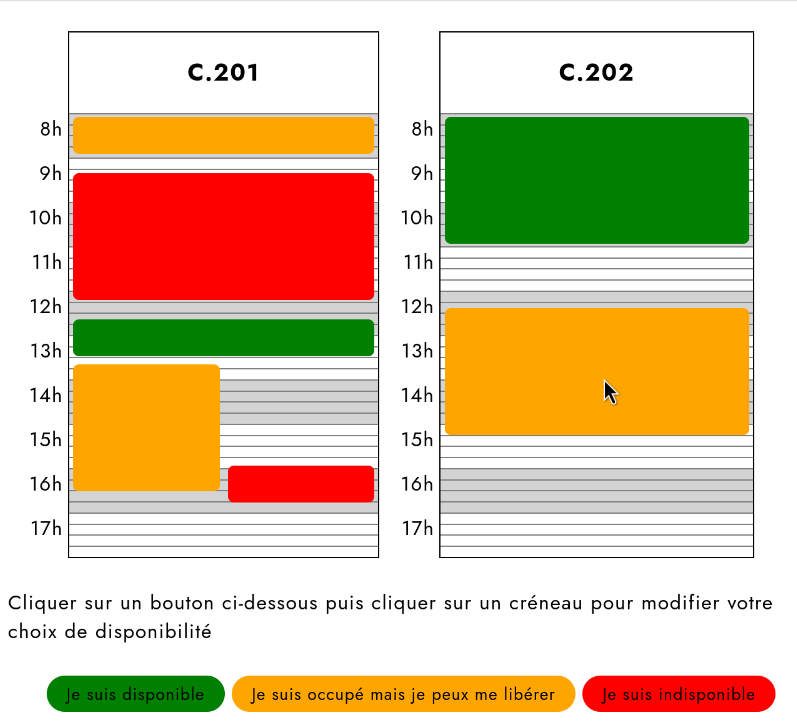
\includegraphics[width=8cm]{rapport/choix_creneau.png}
        \caption{Choix par un utilisateur}
        \label{fig:choix_util}
    \end{figure}

    \begin{figure}[h]
        \centering
        \includegraphics[width=\textwidth]{rapport/schema_donnees.png}
        \caption{Schéma des relations entre les entities beans}
        \label{fig:modif_event}
    \end{figure}
    
\end{document}